\makeatletter
\def\thickhrulefill{\leavevmode \leaders \hrule height 1ex \hfill \kern \z@}
\def\@makechapterhead#1{%
  \vspace*{10\p@}%
  {\parindent \z@ \centering \reset@font
        {\Huge \scshape \thechapter}
        \par\nobreak
        \vspace*{15\p@}%
        \interlinepenalty\@M
        \begin{tabular}{@{\qquad}c@{\qquad}}
          \hline
          \\
          {\Huge \bfseries #1\par\nobreak} \\
          \\
          \hline
        \end{tabular}
    \vskip 100\p@
  }}
\def\@makeschapterhead#1{%
  \vspace*{10\p@}%
  {\parindent \z@ \centering \reset@font
        {\Huge \scshape \vphantom{\thechapter}}
        \par\nobreak
        \vspace*{15\p@}%
        \interlinepenalty\@M
        \begin{tabular}{@{\qquad}c@{\qquad}}
          \hline
          \\
          {\Huge \bfseries #1\par\nobreak} \\
          \\
          \hline
        \end{tabular}
    \vskip 100\p@
  }}

\chapter{Követelmény leírás}
  
\section{Funkcionális követelmények}
\subsection{Felhasználói kezelés} % (fold)
\label{sub:felhasználói}
  \paragraph{Azonosítás} A renszer használatához, felhasználói azonosítás szükséges. Az azonosítás módja a megszokott felhasználói név, vagy email cím valamint jelszó megadásával történik. Megadott számú sikertelen belejelentkezés esetén a felhasználói név vagy email cím letiltása fél vagy több óráig.
  
  
  \paragraph{Session} Sikeres azonosítás után, böngészőben tárolt session ideje alatt lehet a rendszert használni. Session timeout után, újra bekell jelentkeznie.
  
  
  \paragraph{Regisztráció} Új felhasználó esetén felvétele regisztrációval történik, ahol megkell adnia az email címét valamint kívánt jelszavát.
  
  \begin{figure}[h!]
    \centering
    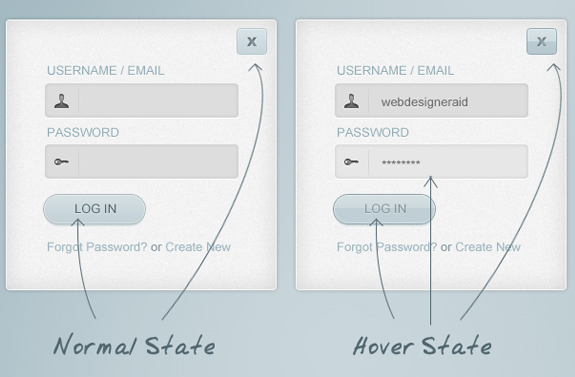
\includegraphics[width=0.6\textwidth]{chapters/chap2/login_sketch.jpg}
    \caption{Bejelentkezés form terv}
  \end{figure}

% subsection felhasználói (end)

\subsection{Kamera kezelés} % (fold)
\label{sub:kamerák_kezelése}

  \paragraph{Felvitel} Egy kamera felviteléhez szükséges adatok:
  \begin{enumerate}
    \item Pozíció (Latitude, Longitude) adat.
    \item Egyedi azonosító, amely egyértelműen meghatározza az felvinni kívánt kamerát.
    \item Pontos cím.
    \item Állapot.
    \item Mobilitás.
    \item Video Stream cím.
  \end{enumerate}
  
  \paragraph{Állapot} Kamera állapota tájékoztatja felhasználót és a karbantartó egységet, hogy javításra szorul-e vagy sem. Állapotai lehetnek:
  \begin{itemize}
    \item Inaktív: Nem elérhető, javításra szorul.
    \item Aktív: Működik.
    \item Hibás: Hardver vagy szoftveres hiba, javításra szorul.
    \item Javítás alatt: Karbantartó egység éppen dolgozik rajta.
  \end{itemize}

  \paragraph{Moblitás} Kamera egy tulajdonsága, amely egyértelműen leírja, hogy ideiglenesen van az adott helyen például egy rendezvény ideje alatt, vagy állandó a pozíciója. Mobilitás tulajdonságából tudhatjuk, hogy milyen célból lett kitelepítve egy kamera.
  \begin{itemize}
    \item Mobil: Ideiglenesen vagy megadott időtartamig van a meghatározott helyen.
    \item Fix: Állandó, objektumok, forgalom megfigyelés szempontjából van.
  \end{itemize}
  
  \paragraph{Video stream} Minden IP alapú kamera multimédia tartalmat továbbít a felhasználó számára, esetünkben legyen ez video alapú hang nélkül. Kamera felvitele során lekell tudnunk ellenőrízni, hogy a video tartalom továbbítás valóban működik-e vagy sem.
  
  \paragraph{Módosítás} Egy kamera módosítása esetén csak a helyzetét, látómezőjét, állapotát, mobilitását és video stream címét lehet megváltoztatni. Azonosítóját nem lehet megváltoztatni, mivel ez alapján tudjuk egyértelműen beazonosítani a rendszerben.
  
% subsection kamerák_kezelése (end)

\subsection{Esemény kezelés} % (fold)
\label{sub:esemény_kezelés}
  Egy esemény megfigyeléséhez több kamera szükséges. Fontos, hogy az adott esemény megtervezésekor előre tudni, hogy mely kamerák szorulnak javításra vagy pozíció változatatásra, esetleges mobil kamerák elhelyezésére.
  Egy eseményben résztvevő kamerák megtekintési sorrendje is nagyon fontos szerepet játszik, azonban a sorrendet változtatni lehet, felmerülő igény esetén.
  
  
  \paragraph{Létrehozás}
  Egy esemény a legtöbb esetben poligonnal ábrázolható. Adott poligon területébe eső kamerákat megkell tudnunk határozni, még mielőtt elmentenénk az eseményt egyébb adataival, amelyek a következőek:
  \begin{enumerate}
    \item Egyedi azonosító.
    \item Megnevezés: kiegészítő információ.
    \item Esemény kezdetének dátuma.
    \item Esemény végének dátuma.
  \end{enumerate}

  \paragraph{Módosítás}
  Egy eseményt csak geometriai tulajdonságát, leírását, kezdeti és vég dátumát lehetséges megváltoztatni.
  
  \paragraph{Megtekintés}
  Megtekintésekor a kamerákat egymás mellett, megadott sorrendben kell megmutatni. Sorrendiségüket bármikor meglehessen változatni, ez a művelet azonban nem számít módosításnak, mivel csak a kamerák megtekintési sorrendiségét változtattuk.
% subsection esemény_kezelés (end)

\subsection{Súgó} % (fold)
\label{sub:súgó}
  Geometriai objektumok felvitele és módosítása nem minden felhasználó számára egyértelmű, ezért egy olyan felületet kell biztosítani, ahol ikon-funkciók levannak írva valamint egy "homokozó" felületet szükséges, ahol kilehet próbálni.
  
  
  Az alkalmazás két fő részből áll:
  \begin{enumerate}
    \item Kamera kezelés
    \item Esemény kezelés
  \end{enumerate}
  Tájékoztató jellegű információval kell biztosítani a felhasználót, hogy melyik lépés után, mit kell végrehajtani, független a felhasználói dokumentációtól.
% subsection súgó (end)

\subsection{Főoldal} % (fold)
\label{sub:főoldal}
  Az alkalmazás belépési pontja, ahonnan kiindulva eltudja érni a kamera kezelés és esemény kezelés funkciókat. Ezenkívül a belépés és regisztráció is ezen a felületen keresztül történik.
% subsection főoldal (end)

	

\section{Nem funkcionális követelmény}
\subsection{Termék követelmény} % (fold)
\label{sub:termék_követelmény}
Az alkalmazás webes alapúnak kell lennie. Firefox, Chrome, Opera, Safari valamint Internet Explorer alatt is működnie kell.
% subsection termék_követelmény (end)

\subsection{Szervezeti követelmény} % (fold)
\label{sub:szervezeti_követelmény}
Felhasznált technológiák csak is kizárólag nyíltforráskódúak legyenek. Kulcs fontosságú az adatbázisrendszer, webes keretrendszer valamint térkép szolgáltató rendszerek nyíltforráskódú vagy ingyenes tulajdonsága.

% subsection szervezeti_követelmény (end)
